% !TEX encoding = UTF-8 Unicode

\documentclass[a4paper]{article}

\usepackage{color}
\usepackage{url}
\usepackage[T2A]{fontenc} % enable Cyrillic fonts
\usepackage[utf8]{inputenc} % make weird characters work
\usepackage{graphicx}
\usepackage{listings}
\usepackage{amsthm}
\usepackage[english,serbian]{babel}
\usepackage[autostyle]{csquotes}
%\usepackage[english,serbianc]{babel} %ukljuciti babel sa ovim opcijama, umesto gornjim, ukoliko se koristi cirilica

\usepackage[unicode]{hyperref}
\hypersetup{colorlinks,citecolor=green,filecolor=green,linkcolor=blue,urlcolor=blue}

\lstMakeShortInline[columns=fixed]|

%\newtheorem{primer}{Пример}[section] %ćirilični primer
\newtheorem{primer}{Primer}[section]
\newtheorem{definicija}{Definicija}[section]

\begin{document}

\title{Kratki vodič kroz Git\\ \small{Seminarski rad u okviru kursa\\Metodologija stručnog i naučnog rada\\ Matematički fakultet}}

\author{Nemanja Radosavljević, Milan Stojković\\ shoocky1337@gmail.com, milanzp@hotmail.com}
\date{9.~april 2016.}
\maketitle

\abstract{

Ovaj rad pokušava da pruži kratak vodič kroz jedan od najčešće korišćenih i najpopularnijih sistema za kontrolu verzija. Git. Rad prolazi kroz osnovne komande i način funkcionisanja Git sistema, na način koji bi trebalo da obezbedi da čitalac po završetku čitanja može da počne sa samostalnim korišćenjem ovog sistema.


\tableofcontents

\newpage

\section{Uvod}
\label{sec:uvod}
Sistemi za kontrolu verzija su jedan od najvažnijih alata pri razvoju softvera. Danas se teško može zamisliti bilo kakav projekat koji ne koristi jedan ovakav sistem. Nažalost, njihovo poznavanje se pretpostavlja, a studenti računarskih nauka se sa njima susreću samo kroz pominjanje.\\ Svrha ovo rada je pre svega upoznavanje citaoca koji nema nikakvo predznanje, ili je ono minimalno, sa osnovnim komandama i nainom funkcionisa sistema Git(u daljem tekstu samo Git). Rad moze da sluzi kao uvod potpunim pocetnicima, ili kao brzi podsednik naprednim korisnicima.\\
U ovom radu se nećemo baviti teorijskim osnovama kontrole verzija, kao što su implementacija praćenja promena, razlike izmedju distribuiranih i centralizovanih sistema itd. Izvori koji sadrže detaljnija objasnjanja, kao i stvari koji su van okvira ovog rada se mogu naći u priloženoj literaturi.\\
Na početku se bavimo životnim ciklusom datoteke koja se nalazi u Git sistemu. Ovaj kratki, i jedini teorijski osvrt u ovom radu predstavlja osnovni preduslov za pravilno razumevanje načina na koji Git prati i čuva promene. Takodje izlažemo osnovnu terminologiju u sistemima za kontrolu verzija, u slučaju da je čitaocu ovo prvi dodir sa temom.\\
Potom se bavimo podešavanjem okruženja za rad.
Ostatak rada je koncipiran tako da se uvode redom osnovne Git komande, zajedno sa definicijom i primerom, na način koji bi po završetku čitanja, stvorio sliku o mogućnostima, efikasnosti i lakoći za rad koju pruža Git.
Za sve primere koristimo komandnu liniju (konzolu). Iako postoji veliki broj grafičkih korisničkih okruženja, oni spadaju van okvira ovog rada, a i sama komandna linija je više nego dovoljna za ilustraciju izabranih tema.

\section{Sekcije Git projekta i životni ciklus datoteke}
\label{zivotni_ciklus}
Pre nego što počnemo sa razmatranjem korišćenja Git sistema bilo bi zgodno uvesti neki osnovne pojmove vezane za kontrolu verzija. Ovo može koristiti korisnicima koji nemaju nikakvog prethodnog iskustva sa sistemima za kontrolu verzija. Sa druge strane, korisnici koji imaju iskustva mogu preskočiti ovaj deo i nastaviti od \ref{subsec:sekcije}. Terminologija varira od sistema do sistema, pa ćemo se fokusariti samo na one univerzalne termine, koji su zajednički za sve sisteme.

\begin{definicija}
Repozitorijum ili baza predstavlja skup svih fajlava koja se nalaze pod kontrolom verzije.
\end{definicija}

\begin{definicija}
Verzija predstavlja sliku stanja sadržaja repozitorijuma u nekom trenutku razvoja.
\end{definicija}

\begin{definicija}
Radna kopija (working copy) predstavlja lokalnu kopiju verzije koja se menja tokom rada.
\end{definicija}

\begin{definicija}
Podizanje promene ili komit (commit) predstavlja akciju kojom se trenutno stanje zapisuje u repozitorijum. Takodje može da se koristi za referisanje odredjene promene.
\end{definicija}

\begin{definicija}
Grana (branch) predstavlja imenovan tok razvoja nezavistan od ostalih tokova.
\end{definicija}
Iako su grane medjusobno nezavisne, one uglavnom imaju zajednički neki deo istorije. Svaka grana pocinje kao kopija neke druge grana i odatle nastavlja da se razvija nezavisno. Početna grana, odnosno ona koja nije nastala kopijom neke druge se sreće pod nazivima trunk, mainline, master.

\begin{definicija}
Konflikt predstavlja situaciju u kojoj dva korisnika pokusavaju da podignu izmenu koja se odnosi na isti deo iste datoteke.
\end{definicija}
Više reči o konfliktima će biti u poglavlju \ref{subsec:konflikti}.


\subsection{Sekcije Git projekta}
\label{subsec:sekcije}
Kako bi se potpuno shvatilo funkcionisanje Git-a, potrebno je razumeti njegove tri sekcije koje koristi za praćenje promena: Radni direktorijum, prostor za pripremu(eng. Staging area) i Git direktorijum odnosno baza. \textbf{Radni direktorijum} sadrži samo jednu verziju datoteka, i to one nad kojima se trenutno radi. To mogu biti datoteke koje ste povukli iz repozitorijuma ili novonapravljene datoteke, sa njima radite, odnosno njih menjate. \textbf{Staging area} je suštinski samo jedna datoteka koja čuva informacije o tome koje ste datoteke označili da želite da budu deo sledećeg komita. \textbf{Git direktorijum} je direktorijum u kom Git čuva sve meta podatke i bazu podataka svih fajlova koji su pod sistemom za kontrolom verzija. Iako postoji način da se datoteke direktno prebace iz radnog u Git direktorijum, to ne umanjuje znacaj sekcije Staging area. Na primer, ukoliko pri razvoju složenene funkcionalnosti napravite ispravnu, stabilnu verziju, medjutim želite da malo eksperimentišete sa njom jer mislite da postoji i bolje rešenje. Ukoliko ste je pre eksperimentisanja prebacili u Staging area, ne postoji bojazan da bilo šta izgubite. Ako eksperimentisanje dovede do toga da je datoteka bespovratno uništena, i dalje postoji ispravna verzija u Staging area koja se može komitovati.\\
Sa ovime u vidu, koraci u okviru jednog komita bi izgledali ovako.
\begin{enumerate}
\item Izmena datoteka
\item Odabir koje datoteke će učestvovati u sledećem komitu i njihovo prebacivanje u Staging Area
\item Komitovanje
\end{enumerate}

Posle svakog komita sadržaj radnog i Git direktorijuma je isti i ciklus se može ponovo započeti. Ilustracija ovih koraka je prikazana na slici \ref{fig:git_sekcije}.\\
Pored ovog smera kretanja kroz Git sekcije, mogući su i drugi, koji se koriste radi ispravljanja grešaka i njima se bavimo u poglavlju \ref{subsec:greske}

\begin{figure}[h!]
\begin{center}
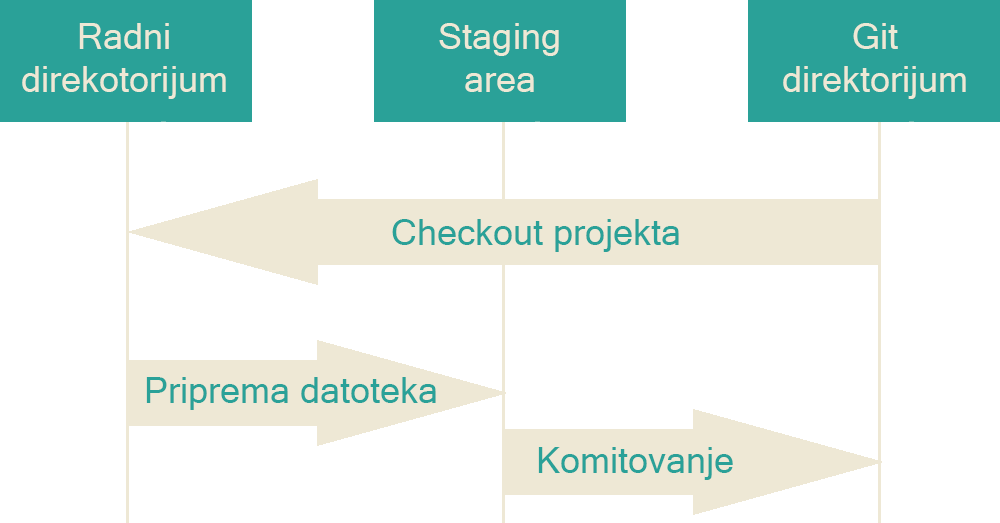
\includegraphics[scale=0.19]{images/sekcije.png}
\end{center}
\caption{Sekcije Git-a}
\label{fig:git_sekcije}
\end{figure}



\subsection{Životni ciklus datoteke}
\label{subsec:ciklus}
Datoteke u radnom direktorijumu pre svega mogu biti \textbf{praćene} i \textbf{nepraćene}. Izrazi praćene i nepraćene nam suštinski govore da li se te datoteke u poslednjoj verziji nalaze pod sistemom za kontrolu verzija.\\
One koju su \textbf{praćene} mogu biti \textbf{modifikovane, nemodifikovane} i \textbf{spremne za komitovanje (staged).} Pri prebacivanju datoteka iz Git direktorijuma u radni ili pri kloniranju repozitorijuma, datoteke u radnom direktorijumu imaju status \textbf{nemodifikovane}. Menjanjem istih, Git ih prepoznaje kao \textbf{modifikovane} jer više nisu iste kao poslednja komitovana verzija. Označavanjem da je neka datoteka spremana za komitovanje i komitovanjem, životni ciklus te datoteke se zatvara. Verzija u radnom direktorijumu više nije različita od poslednje komitovane verzije, pa ta datoteka ponovo imas status nemodifikovane.
\textbf{Nepraćene} datoteke, pored toga što mogu nastati pravljenjem novih datoteka, mogu biti i datoteke koje su bile pod sistemom za praćenje verzija, ali su obrisane odatle. Uvođenje nepraćenih datoteke pod sistem za kontrolu verzija započinje tako što se one označe kao spremne za komitovanje, a onda se mogu komitovati i time postaju praćene.
Ilustracija se može videti na slici \ref{fig:git_lifecycle}.

\begin{figure}[h!]
\begin{center}
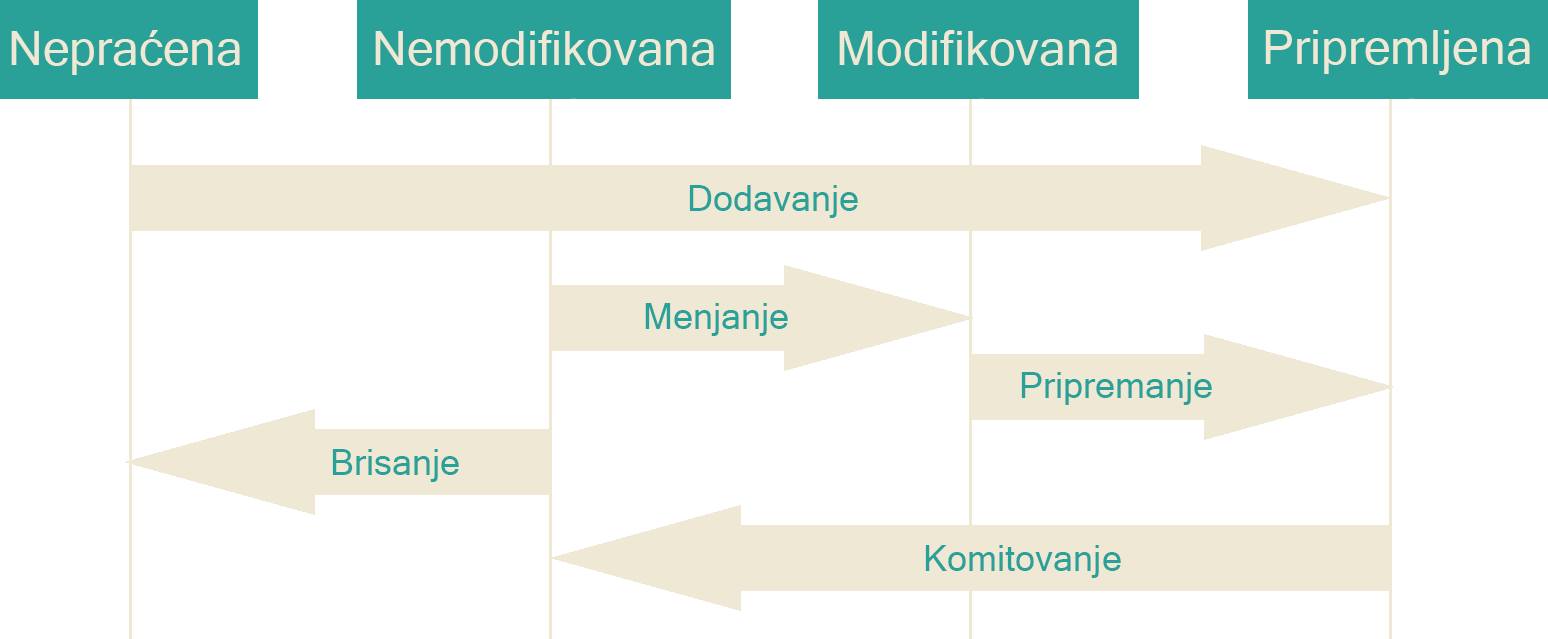
\includegraphics[scale=0.18]{images/lifecycle2.png}
\end{center}
\caption{Životni ciklus datoteke u Git-u}
\label{fig:git_lifecycle}
\end{figure}


\section{Kreiranje repozitorijuma i osnovne komande}
\label{sec:kreiranje}

Kako bi Git mogao da prati ko je napravio izmene, potrebno je da mu se predstavite. Izmedju ostalog, za to koristimo  |git config| komandu.

\begin{lstlisting}[language=bash]
git config --global user.name <name>
git config --global user.email <email>
\end{lstlisting}

\noindent
Podešavanje imena korisnika je obavezno, jer se svaki komit vezuje za korisnika koji ga je napravio. Opcija |--global| označava da je podešavanje globalnog opsega, tj. važi za sve repozitorijume u sistemu. Izostavljanjem ove opcije podešavanje se vezaju samo za tekući repozitorijum. Sva podešavanja sa globnim opsegom se čuvaju u \textit{.gitconfig} datoteci u \textit{home} direktorijumu na Linux sistemima. Direktnim menjanjem sadržaja ove datoteke se može izbeći kucanje komandi za svako podešavanje koje želimo da promenimo. Dodatne informacije o |git config| komandi kao i neka zgodna podešavanja se mogu naći u literaturi.

\subsection{Osnovne komande}
\label{osnovne_komande}

\subsubsection*{git init, git clone}
\label{subsec:git_init}
Git repozitorijum se može inicijalizovati u praznom direktorijumu, ali i u direktorijumu u kom se već radi na projektu. Za ovo se koristi komanda |git init|. Time će biti napravljen direktorijum \textit{.git} koji sadrži meta podatke repozitorijuma i pored toga sve ostalo ostaje nepromenjeno. Primer inicijalizacije repozitorijuma moze se videti na slici \ref{fig:git_init}.

U velikoj većini slučajeva, |git init| se poziva samo jednom, za pravljanje centralnog repozitorijuma. Kasnije, svi oni koji učestvuju u razvoju će taj repozitorijum kopirati na lokalne mašine pomoću komande:
\begin{lstlisting}[language=bash]
git clone <repozitorijum>
\end{lstlisting}
\noindent
gde |<repozitorijum>| treba zameniti adresom ogriginalnog repozitorijuma. Lokalni repozitorijum ima svoju istoriju izmena, svoje fajlove i potpuno je nezavisno okruženje od originalnog repozitorijuma. 

\begin{figure}[h!]
\begin{center}
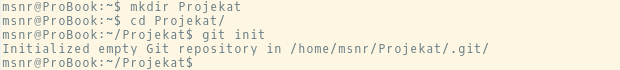
\includegraphics[scale=0.55]{images/init.png}
\end{center}
\caption{Inicijalizacija Git projekta u novonapravljenom direktorijumu}
\label{fig:git_init}
\end{figure}


\subsubsection*{git status}
\label{subsec:git_status}
Provera koje su to datoteke spremne za komitovanje (Staging Area) može se uraditi komandom |git status|. Pored toga, korišćenjem iste komande prikazuje se koje su datoteke promenjene u odnosu na repozitorijum, ali nisu spremne za komitovanje, kao i datoteke koje ne postoje u repozitorijumu, odnosno sistem za kontrolu verzija ih i dalje ne prati.

\subsubsection*{git add}
\label{subsec:git_add}
Nakon izmena u radnoj verziji koje želite da upišete u repozitorijum, potrebna je priprema tih datoteka, odnosno dodavanje datoteka u Staging Area. Priprema za komitovanje se vrši komandom |git add| koja može bit pozvana više puta pre komitovanja, za istu ili neku drugu datoteku.


\subsubsection*{git commit}
\label{subsec:git_commit}
Upisivanje promena u repozitorijum, odnosno komitovanje, zahteva od korisnika i poruku kojom opisuje promene. Pozivom |git commit| komande otvara se podrazumevani tekst editor gde je potrebno uneti opis, a nakon toga se komit čuva u repozitorijumu. Opcijom -m i navođenjem poruke nakon nje se naznačava da želimo da koristimo tu poruku kao opis i tada se ne otvara tekst editor.
\\\\
Svaki komit u bazi je jedinstveno odredjen SHA-1 heš vrednošću. Za referisanje se najčesće koristi skraćena verzija, odnosno prvih 7 karaktera (npr. 6cfaf1c).
Takodje, radi lakšeg referisanja uvedena su specijalna imena za odredjene komitove. Jedan od njih je HEAD. HEAD predstavlja poslednji komit na grani na kojoj se nalazimo. Dodatno se može koristiti i HEAD\^{}n za referisanje n-tog pretka HEAD komita.\\
Bitno je napomenuti da pored izmena iz kojih se sastoji svaki komit, on sadrži i pokazivač na komit koji mu prethodi. Ovaj mali detalj će nam omogućiti lakše shvatanje kako Git vodi računa o granama.\\
Na slici \ref{fig:git_commit} je prikazan primer pripreme, komitovanja i pregleda statusa datoteka tokom ovog procesa.


\begin{figure}[h!]
\begin{center}
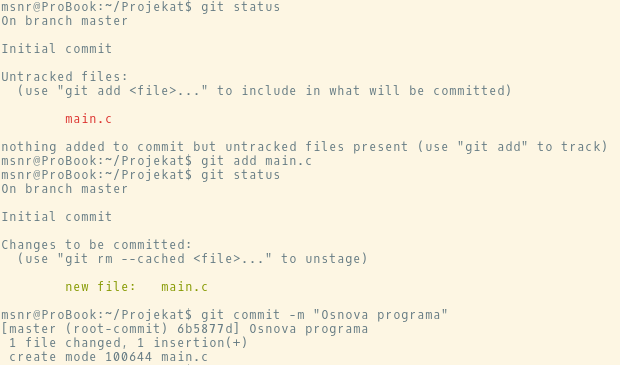
\includegraphics[scale=0.55]{images/commit.png}
\end{center}
\caption{Priprema i komitovanje novog fajla, pregled statusa tokom procesa}
\label{fig:git_commit}
\end{figure}

\subsubsection*{git log}
\label{log}
Komanda |git log| se koristi za izlistavanja detalja o postojećim komitovima. Osnovni format je štur, a može biti i prilično nepregledan ako nas zanima veći broj komitova ili sam razvoj grane. Srećom, ova komanda ima mnoštvo dodatnih opcija i može se koristiti na razne načine. Neke od korisnijih opcija su navedene u tabeli \ref{tab:tabela1}.. 

\begin{table}[h!]
\begin{center}


\begin{tabular}{cc} \hline
komanda & opis\\ \hline
-n <number> & ograničava broj prikazanih komitova na <number> \\
--skip=<number> & preskače <number> komitova pre početka izlistavanja \\
--since=<date> & prikazuje komitove nastale posle <date> \\
--author=<author> & prikazuje komitove navedenog autora \\
--format=<format> & detaljno formatiranje (pogledati man stranice)
\end{tabular}
\caption{Neke od opcija git log komande}
\end{center}
\label{tab:tabela1}

\end{table}


\subsubsection*{git diff}
\label{subsec:git_diff}
Komanda |git diff| podrazumevano ispisuje razliku izmedju radnog direktorijuma i Staging area. 
Ako se navede HEAD ili identifikator nekog drugog komita, prikazaće se razlika izmedju radnog direktorijuma i traženog komita. Opcijom |--cached| se označava da nas zanima razlika izmedju Staging Area i poslednjeg komita.
Izlaz |git diff| komande je sličan diff naredbi na Linux-u, a detalji se mogu naći u \cite{pocketguide} u poglavlju 11.


\subsubsection*{git checkout}
\label{checkout}
Komanda |git checkout <file | branch | commit>| se koristi za menjanje radne kopije verzijom iz repozitorijuma. Specijalni slučaj korišćenja ove komande se odnosi na rad sa granama i objašnjen je u poglavlju \ref{subsec:pravljenje_grana}\\
Ukoliko se navede ime datoteke sadržaj te datoteke u radnoj kopiji će biti zamenjem sadržajem te datoteke iz repozitorijuma, dok ukoliko se navede ime grane, sadržaj kompletnog radnog direktorijuma će biti zamenjem sadržajem grane iz repozitorijuma.\\
U slučaju da se navede identifikator komita, dobiće se slika repozitorijuma koja odgovora tom komitu. Tada će se radni direktorijum nalaziti u ``detached HEAD'' stanju, tj. moguće je samo pogledati stanje, ne i menjati ga. Da bi se nastavilo sa menjanjem mora se preuzeti sadržaj neke grane.

\subsection{Ispravljanje grešaka}
\label{subsec:greske}

U zavisnosti od toga u kom se stanju nalazi fajl koji sadrži grešku koji želimo da ispravimo, ispravljanje grešaka možemo svrstati u četiri kategorije. One su redom: ispravljanje lokalnih grešaka, ispravljanje grešaka koje se nalaze u Staging Area, ispravljanje komitovanih grešaka i uklanjanje kompletnih komitova.

\subsubsection*{Ispravljanje lokalnih grešaka}
\label{lokalne_greske}
Pretpostavimo da smo napravili grešku koju jos nismo ni pripremili za komit, niti je komitovali, a pritom želimo da je ispravimo. Tacnije, želimo da se vratimo na stanje koje je bilo pre naših izmena. Već smo se upoznali sa komandom checkout i jasno je da ona može da se iskoristi i za ovakvu situaciju. Dakle, dovoljno je komandom |git checkout| dovući poslednju ispravnu verziju datoteke koja nam je potrebna.

\subsubsection*{Ispravljanje grešaka u Staging Area}
\label{staging_greske}

Pretpostavimo da smo napravili dobru izmenu, pripremili je za sledeći komit, a potom shvatili da smo ipak napravili grešku, i da ili želimo da dodamo jos neku izmenu ili da potpuno odustanemo od izmena. Za ovo je potrebno osloboditi Staging area komandom |git reset HEAD|. Ako se dodatno navede ime datoteka, samo ona će biti izbrisina iz Staging Area.

\subsubsection*{Ispravljanje komitovanih grešaka}
\label{komitovane_greske}
Do sada smo videli kako da ispravimo greške koja su nastale pre trajnog zapisivanja u repozitorijum. Postavlja se pitanje šta uraditi ako smo neke neželjene promene trajno zapisali, a želimo da ih ispravimo. Ovo je moguće postići na dva načina: korišćenjem |git revert <commit>| komande, i korišćenjem |git reset <commit>| komande sa opcijom |--hard|.\\
|git revert| uvodi novi komit koji otklanja promene nastale komitom koji želimo da ispravimo, dok korišćenje |git reset| komande sa opcijom |--hard| trenutna grana će imati vrednost navedenog komita, i svi komitovi nastali posle njega će se izgubiti. \\

Prvi način je bezbedan, ali ružan. Umesto da eliminišemo neželjeni komit zapravo dobijamo dva komita koja se odnose na grešku. Drugi slučaj lepši ali ``prljaviji'', jer zapravo menjamo tok istorije repozitorijuma što nekad nije poželjno raditi, pogotovo kad su u pitanju udaljeni repozitorijumi. \\

Ukoliko ne želimo da obrišemo kompletne promene uvedene komitom, već želimo da dodamo nešto što smo zaboravili ili da promenimo poruku, može se iskoristi |git commit| sa opcijom |--amend|  koja će dodatne izmeni samo dodata kao sastavni deo poslednjeg komita. Efekat ove komande je identičan kao da smo resetovali granu na prethodni komit, i napravili novi koji sadrži potpunu izmenu.


\section{Rad sa granama}
\label{sec:grane}
Grananje predstavlja razdvajanje toka razvoja kako bi se radilo na stvarima za koje se još ne zna da li mogu narušiti trenutno stanje ili uvesti neželjene promene. Zgodne su za eksperimentisanje i nezavistan razvoj dodatnih mogućnosti bez bojazni da će nešto krenuti po zlu. Jednostavno, rad na jednoj grani ne utiče na ostale.\\
Git je implementiran tako da je rad sa granama prirodan, brz i veoma efikasan i stoga se njihovo korišćenje ohrabruje. Za razliku od drugih sistema za kontrolu verzija, grana u Git sistemu predstavlja jednostavan pokazivač na odredjeni komit. Znači pravljenje grana predstavlja akciju pravljenja dodatnog pokazivača, razvoj grane dodavanje novih komitova i pomeranje ovog pokazivača na najnoviji, a brisanje grana brisanje pokazivača.

\subsection{Pravljenje i praćenje grana}
\label{subsec:pravljenje_grana}
Za pravljenje nove grane koristimo opciju |git branch <ime grane>|. Bitno je napomenuti da smo ovimo samo napravili novi pokazivač, i da se i dalje nalazimo na istoj grani na kojoj smo bili. Da bismo se prebacili na novokreiranu granu potrebno je uraditi |git checkout <ime grane>|. Da ne bi koristili dve komande za pravljenje i prebacivanje na novu granu, ovo je moguće uraditi jednom komandom: |git checkout -b <ime grane>|. 
Sada, kada se nalazimo na novoj grani, svako dodavanje komita će zajedno sa pomeranjem našeg HEAD pokazivača, istovremeno pomerati i pokazivać koji odgovara grani na kojoj se nalazi. Skakanje sa grane na granu se može zamisliti jednostavnim menjanjem HEAD pokazivača, vrednošći pokazivača koji odgovara grani na koju želimo da skočimo.\\
Za brisanje grana se koristi komanda |git branch -d <ime grane>|. Sve što će uraditi ova komanda je obrisati pokazivač tako da mi više nemamo uvid u njeno postojanje. Postavlja se pitanje da li će Git obrisati i sve komitove koje pripadaju samo obrisanoj grani? Neće. Ovo je još jedna od zgodnih strana Git-a, koji zapravo ništa ne briše kompletno, već samo nama nedozvoljava da direktno vidimo ``obrisane'' stvari. One se i dalje nalaze u \textit{.git} direktorijumu, i za trajno brisanje podataka je potrebno ručno obrisati ih u njemu. Detalji o tome kako pronaći ovakve promene se nalaze u \cite{progit}.\\\\
Kada završimo sa razvojem naše grane i ispostavi se da nam razvijeni dodaci odgovoraju, poželjno je da imamo mogućnost da ih integrišemo sa sadržajem naše glavne grane. U Git-u je ovo moguće uraditi na dva različiti načina korišćenjem dve komande:|git rebase| i |git merge|.  

\subsection{Rebase}
\label{subsec:rebase}
Rebase predstavlja akciju integrisanja razlika izmedju trenutne grane i neke druge, tačnije pomerenje komita u kom su se grane razdvojile na najsvežiji komit grane sa kojom se vrši integracija.\\
Ovo se postiže komandom |git rebase <ime grane>|. Rezultat ove operacije je ilustrovan na slici \ref{fig:rebase}. Prvobitno je komit u kome su grane razdvojile bio K5. Grane su se nezavisno razvijale i u jednom trenutku je pozvan rebase sa namerom da se promene nastale na master grani integrišu u eksperimentalnu granu. U trenutku pozivanja komande rebase, prvo što Git uradi je pronalaženje zajedničkog pretka dveju grana (u ovom slučaju K4). Potom privremeno čuva sve komitove nastale od tog trenutka na grani na kojoj se nalazimo (Eksperiment), i pomera trenutnu granu na granu koju integrišemo (K5), tako da je sad prvi zajednički predak K5. Nakon ovog dodaje sve privremeno sačuvane komitove i pomera pokazivač trenutno grane na poslednji. Ovime je proces rabase završen.
\begin{figure}[h!]
\begin{center}
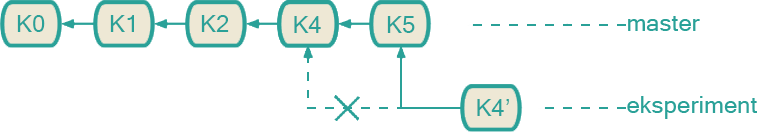
\includegraphics[scale=0.3]{images/rebase.png}
\end{center}
\caption{Ilustracija procesa spajanja}
\label{fig:rebase}
\end{figure}

\subsection{Merge}
\label{subsec:merge}
Merge ili spajanje predstavlja akciju spajanja istorije dve grane, tako da posle spajanja pokazuju na isti komit. Ovo se postiže komandom |git merge <ime grane>|. Rezultat ove operacije je ilustrovan na slici \ref{fig:merge}. U trenutku poziva ove komande Git pronalazi najnovije komitove grana koje učestvuju u spajanju kao i njihovog zajedničkog pretka. U ovom slučaju to su redom, K2, K3 i K4. Potom pravi novi komit kao razliku ova tri komita i dodaje ga kao novi komit master grane (K5). Sada master sadrži sve promene koje se nalaze u ekperimentalnoj grani i ona se po potrebi može obrisati.
\begin{figure}[h!]
\begin{center}
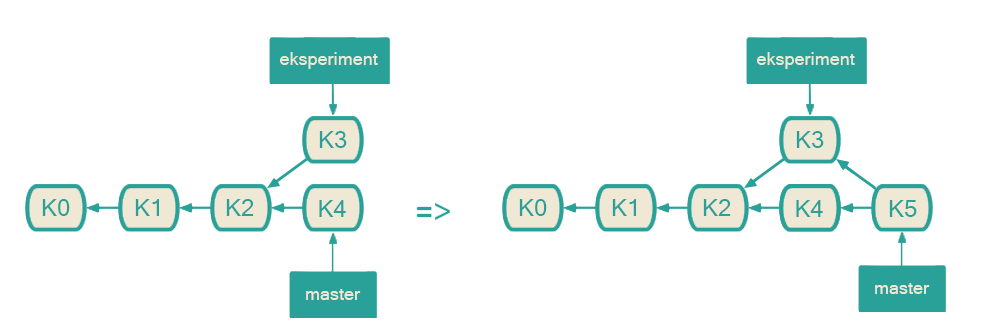
\includegraphics[scale=0.3]{images/merge.png}
\end{center}
\caption{Ilustracija procesa spajanja (pre i posle spajanja)}
\label{fig:merge}
\end{figure}

\subsection{Konflikti}
\label{subsec:konflikti}
Jedna od najverovatnijih stvari koja će se desiti pri spajanju ili rebase procesu je da će nastati konflikt. Konflikt predstavlja situaciju u kojoj Git nije u stanju da razazna čiju verziju treba da primeni. Kada dodje do konflikta Git prekida sa ovim akcijama, upisuje izmene obe strane i traži od korisnika da ručno razreši konflikt pre nego što nastavi. Mesto gde je nastao konflikt se može prepoznati po tome što se u datoteci koju Git prijavi kao problematičnu nalaži sledeći segment:
\begin{lstlisting}
<<<<<<<<<<< HEAD
tekst
===========
tekst
>>>>>>>>>>> SHA-1 komita
\end{lstlisting}
Prvi deo, izmedju markera ``|<<<<<<|'' i ``======'' sadrži promene nastale u trenutnoj grani. Deo zmedju  ``======'' i ``|>>>>>>|'' sadrži promene nastale u grani sa kojom se pokušava spajanje ili rebase. Sve što korisnik treba da uradi je da obriše ove markere, odluči koje stvari želi da zadrži i potom komituje razrešenu verziju i nastavi sa željenom akcijom.
\section{Rad sa udaljenim repozitorijumima}
\label{sec:udaljeni_repozitorijumi}
Rad sa udaljenim repozitorijumima je gotovo neizbežan u korišćenju Git-a, no, obzirom da postoji nezavisan lokalni repozitorijum, to je prilično jednostavno. Potrebno je osvežiti sadržaj lokalnog repozitorijuma iz udaljenog, odnosno propagirati promene u udaljeni repozitorijum.


\subsection{git fetch i git pull}
\label{subsec:git_pull}
Izmene sačuvane u udaljenom repozitorijum mogu se povući i u lokalni komandom |git fetch|. Medjutim, ova komanda ne osvežava i sadržaj radnog direktorijuma, već samo lokalnog repozitorijuma, a onda je na vama da to spojite sa izmenama u radnom direktorijumu. Ono što donekle ubrzava i olakšava ovaj proces je komanda |git pull|. Ona će za vas povući izmene iz udaljenog repozitorijuma i spojiti ih sa izmenama u radnom direktorijumu. Iako u velikoj većini slučajeva ovo radi sasvim dobro, treba ga koristiti s pažnjom jer ne postoji način da vidite koje su to izmene upravo napravljene u radnom direktorijumu i lokalnom repozitorijumu.




\subsection{git push}
\label{subsec:git_push}
Slanje izmena komitovanih u lokani repozitorijum i deljenje sa timom u udaljenom repozitorijumu se ne vrši automatski, već se to mora uraditi ručno, unošenjem komande |git push|. Dodatno, navođenjem |<remote>| i |<branch>| nakon komande, može se precizirati na koji udljeni repozitorijum želite da pošaljete svoje izmene i na koju granu. Pravilo je da se pre slanja izmena u udaljeni repozitorijum, osveži sadržaj lokalnog, jer postoji mogućnost da su u međuvremenu propagirane dodatne izmene. Tada je na vama da sredite konflikte, ponovo povučete promene iz udaljenog repozitorijuma i ukoliko nije bilo nikakvih izmena, tada možete komandom |git push| poslati svoje izmene.



\section{Zaključak}
\label{sec:zakljucak}
Upoznavanjem sa osnovama funkcionisanja Git-a, komandama i nekim njihovim osnovnim opcijama, kao i prikazanim primerima, čitaocima Git više nije nepoznanica. Poznavanje Git-a će im umnogome olašati razvoj softvera u timu i ovaj rad im daje dobru osnovu za to. Time što se nije ulazilo u detalje, olakšava se upoznavanje sa osnovama, ali i ostavlja prostor za dalje upoznavanje sa mnogobrojnim opcijama komandi čijim korišćenjem rad sa Git-om može biti udobniji.

\addcontentsline{toc}{section}{Literatura}
\appendix
\bibliography{seminarski} 
\bibliographystyle{plain}


\end{document}
